\documentclass{article}
\usepackage[pdftex]{color,graphicx}
\usepackage{amsmath}
\usepackage{amssymb}
\usepackage{caption}
%\usepackage{pdfpages}
%\usepackage{listings}
%\usepackage{algorithm}
%\usepackage{algpseudocode}
%\usepackage{algorithmic}
\usepackage{enumerate}
\usepackage{syntonly}
\usepackage{multicol}
\usepackage{array}
\usepackage{mathrsfs}  
 \usepackage[linesnumbered,ruled,vlined]{algorithm2e}
%\usepackage[tight,footnotesize]{subfigure}
%\usepackage{stfloats}
%\usepackage{url}
%\usepackage{threeparttable}
%\usepackage{cite}
\usepackage{exam}
\usepackage{listings}
\usepackage{subcaption}
\usepackage{bm}
%\usepackage{algorithmic}

%**********************************************************************************
% User define command
%**********************************************************************************



\newcommand{\vect}[1]{\mathbf{#1}}
\newcommand{\vectC}[2]{{#1}_{#2}}
\newcommand{\mat}[1]{\mathbf{#1}}
\newcommand{\set}[1]{\mathcal{#1}}
\newcommand{\setE}[2]{{#1}_{#2}}
\newcommand{\setI}[2]{{#1}^{#2}}
\newcommand{\given}{\;\middle|\;}  % This appears with \left(  A \given B \right)
\newcommand{\setcard}[1]{\left\vert{#1}\right\vert}  
\newcommand{\hd}{\mathrm{HD}} 
\newcommand{\hdf}[1]{h_d(#1)} 
\newcommand{\hw}{\mathrm{HW}} 
\newcommand{\hwf}[1]{h_w(#1)} 
\newcommand{\pr}{\mathrm{Pr}}
\newcommand{\chosenr}{\xleftarrow{}}
\newcommand{\dist}[1]{\mathcal{#1}}

\newcommand{\etal}{\textit{et al.~}}
\newcommand{\pc}{\mathrm{PC}}
\newcommand{\hdt}{\mathrm{HDT}}
\newcommand*\diff{\mathop{}\!\mathrm{d}}
\newcommand{\var}{\mathrm{Var}}
\newcommand{\expe}{\mathrm{E}}
\newcommand{\trans}{^\mathsf{T}}


\newenvironment{myenumerate}{
\begin{enumerate}
  \setlength{\itemsep}{4pt}
  \setlength{\parskip}{4pt}
  \setlength{\parsep}{4pt}
}{\end{enumerate}}

%\usepackage{algorithm}
%\usepackage{algcompatible}

% \algblockdefx{FORALLP}{ENDFAP}[1]%
%   {\textbf{for all }#1 \textbf{do in parallel}}%
%   {\textbf{end for}}

\paper{CS60004}  % <- do not include FC, FT etc
%\version{0}                     % <- for multiple choice exams
\subject{CS60004: Hardware Security}
\title{End Semester Examination}
\time{3}                      % <- number of hours: default is three
\semester{Spring}
\year{2018}                     % <- default is the current year
%\campus{Shanghai}
\fullmarks{60}

\note{{\bf {\underline{THIS QUESTION PAPER HAS A CHOICE!}} Questions 1 and 2 are compulsory. However, you 
are supposed to answer only one out of questions 3 and 4. \newline
}}

\begin{document}
\vspace*{-0.3in}
\begin{questions}

\question 

Consider the following algorithm for computing 
modular exponentiation used in the RSA cipher. 
Our objective is to ascertain the scalar $k$ using 
side-channel analysis.\\

\begin{algorithm}[H]

 %\begin{tiny}
   \caption{RSA Modular Exponentiation}
   \label{algo:2}
   \KwData{Base: $X$, Secret Exponent $k=k_{n-1},k_{n-2},\ldots,k_0$ and modulus $N$}
    \KwResult{$Q=X^k$}
   
{$R_0 \rightarrow 1$ ; $R_1 \rightarrow X$ \; }
\For{$i = n-1$ downto $0$}{
{$R_{[1-k_i]} \rightarrow (R_0 \times R_1$) mod $N$\; }
{$R_{k_i} =(R_{k_i}^2$) mod $N$ ; }}
{return $Q=R_0$ \; }
   
%\end{tiny}
  \end{algorithm}
  
You are also given the power trace values of the $10$ exponentiations with different values of the 
base $X$, for 8 leakage points, as shown in Table 1. The value of $N$ is $4763$. 

You are given that the value of $(n-1)^{th}$ bit of $k$ is 1. Find out the value of $(n-2)^{th}$ bit of the $k$ using {\sf Correlation Power Analysis} (CPA). Assume that the leakage model is Hamming weight.

\begin{table}[h]
\scriptsize
\centering
\caption{Power Trace Value of RSA execution}
\begin{tabular}{|c|c|c|c|c|c|c|c|c|c|}
\hline
Execution & $X$ & Leakage  & Leakage  & Leakage & Leakage& Leakage & Leakage& Leakage & Leakage   \\
No       &     & of $(n-1)^{th}$  & of $(n-2)^{th}$ & of $(n-3)^{th}$ & of $(n-4)^{th}$ & of $(n-5)^{th}$ & of $(n-6)^{th}$ & of $(n-7)^{th}$& of $(n-8)^{th}$ \\ 
        &      &    bit        & bit     &  bit    &   bit   &  bit   & bit    & bit    & bit  \\                                                       \hline
1  & 810 & 13 &12 &9 & 12& 11& 12 &10 &7 \\ \hline
2 & 891 & 15 & 13 &7 &14 &9 &17 &11 &11 \\ \hline
3 & 789 &10 &11 &13 &9 &12 &14 &16 & 8 \\ \hline 
4 & 431 & 8 &8 &6 &6 &12 &13 &10 &13 \\ \hline
5 & 918 & 11 & 10 & 9 &9 & 13 &11 &13&13 \\ \hline
6 & 862 & 8 & 6 &6&12 &10 &10 &13 &9 \\ \hline
7 & 706 & 8 & 9 &13 &16 &15 &7 &12 &13 \\ \hline
8 &742 &11 &11 &13 &14 &19 &7 &14 & 12 \\ \hline
9 & 53& 12& 12&15&8&14&12&12&12 \\ \hline
10 & 408 &10&14&10&12&10&19&11& 10 \\ \hline
\end{tabular}
\end{table}

\marks{20}

\question Consider the implementation of binary extended Euclidean algorithm to compute the 
gcd of two numbers $u$ and $v$, as below.

\begin{lstlisting}[language=C]
unsigned int gcd(unsigned int u, unsigned int v)
{
    // simple cases (termination)
    if (u == v)
        return u;

    if (u == 0)
        return v;

    if (v == 0)
        return u;

    // look for factors of 2
    if (u & 1==0) // u is even
    {
        if (v & 1==1) // v is odd
            return gcd(u >> 1, v);
        else // both u and v are even
            return gcd(u >> 1, v >> 1) << 1;
    }

    if (v & 1==0) // u is odd, v is even
        return gcd(u, v >> 1);

    // reduce larger argument
    if (u > v)
        return gcd((u - v) >> 1, v);

    return gcd((v - u) >> 1, u);
}
\end{lstlisting}


The algorithm has been shown in C-language. This code is 
recursive and not constant-time. As you can 
see that the timing would vary and depend on the 
input parameters, thus offering a side-channel 
of the parameters through timing. In order to convert this code 
to a constant time implementation answer the 
following questions:

\begin{enumerate}
\item Convert this recursive implementation of GCD to an iterative algorithm which is free from recursive function calls. Complete the 
following code snippet using the comments as hints.

\marks{10}

% \begin{lstlisting}[language=C]
% unsigned int gcd(unsigned int u, unsigned int v)
% {
%   int shift;

%   /* GCD(0,v) == v; GCD(u,0) == u, GCD(0,0) == 0 */
%   if (u == 0) return v;
%   if (v == 0) return u;
 
%   /* Let shift := lg K, where K is the greatest power of 2
%         dividing both u and v. */
%   for (shift = 0; ((u | v) & 1) == 0; ++shift) {
%          u >>= 1;
%          v >>= 1;
%   }
 
%   while ((u & 1) == 0)
%     u >>= 1;
 
%   /* From here on, u is always odd. */
%   do {
%        /* remove all factors of 2 in v -- they are not common */
%        /*   note: v is not zero, so while will terminate */
%        while ((v & 1) == 0)  /* Loop X */
%            v >>= 1;

%        /* Now u and v are both odd. Swap if necessary so u <= v,
%           then set v = v - u (which is even). For bignums, the
%           swapping is just pointer movement, and the subtraction
%           can be done in-place. */
%        if (u > v) {
%          unsigned int t = v; v = u; u = t; // Swap u and v.
%        }
       
%        v = v - u; // Here v >= u.
%      } while (v != 0);

%   /* restore common factors of 2 */
%   return u << shift;
% }

% \end{lstlisting}

\begin{lstlisting}[language=C]
unsigned int gcd(unsigned int u, unsigned int v)
{
  int shift;

  /* GCD(0,v) == v; GCD(u,0) == u, GCD(0,0) == 0 */
  /*----------Enter your code here-----------*/
 
  /* Let shift := lg K, where K is the greatest power of 2
        dividing both u and v. Compute shift*/
  /*----------Enter your code here-----------*/
 
  while ((u & 1) == 0)
    u >>= 1;
 
  /* From here on, u is always odd. */
  do {
       /* remove all factors of 2 in v -- they are not common */
       /*   note: v is not zero, so while will terminate */
       /*----------Enter your code here-----------*/

       /* Now u and v are both odd. Swap if necessary so u <= v,
          then set v = v - u (which is even).  */
       /*----------Enter your code here-----------*/
       
     } while (v != 0);

  /* restore common factors of 2 and return*/
 /*----------Enter your code here-----------*/
}

\end{lstlisting}



\item Convert the iterative implementation as constructed in the previous question to a constant-time implementation ie, free from if-else structure. (Consider the worst case run-time of the algorithm and make your algorithm run with same execution time irrespective of the input to the algorithm). 
You can assume that the maximum input size is 32 bits. 

\marks{15}

\begin{lstlisting}[language=C]
unsigned int gcd(unsigned int u, unsigned int v)
{
	int shift=0;
	int uval,vval;
	int retu,retv,orgu,orgv;
	/*save the original inputs incase one of the argument is 0 */
	retu = (u == 0) ? 1:0;
	retv = (v == 0) ? 1:0;
	orgu = u;
	orgv = v;
 
	/*Calculate the shift := lg K, where K is the greatest power of 2 
    dividing both u and v, Compute shift in worst-case time*/
	for (int i = 0; i < 32; i++) {
		uval = u;
		vval = v;
         
         /*----------Enter your code here-----------*/
		
	}
    /*Remove powers of 2 from u in worst case time */
	for (int i = 0; i < 32; i++) {
		uval = u;
	   /*----------Enter your code here-----------*/
	}



	
    /* From here on, u is always odd.*/
	for(int i = 0; i< 32; i++)
	{
		/*copy u and v values in temporary variables */
		uval = u;
		vval = v;
		/*remove all factors of 2 in v in worst case time*/
		for (int i = 0; i < 32; i++) {
	    /*----------Enter your code here-----------*/
		}
		/*swap intermediate temporary values of u and v*/
		int utmp,vtmp;
		utmp = uval;
		vtmp = vval;
		 /*----------Enter your code here-----------*/

		/*Update u and v with the temporary values calculated, 
        if (v != 0)*/
		u = (vval != 0) ? uval : u;
		v = (vval != 0) ? vval : v;
	}

	/*Calculate the final return value, handle all cases so that 
    overall run-time is also worst-case and hence constant time*/
    
	
	int final;
	 /*----------Enter your code here-----------*/
	return final;
}
\end{lstlisting}

% \begin{lstlisting}[language=C]
% unsigned int gcd(unsigned int u, unsigned int v)
% {
% 	int shift=0;
% 	int uval,vval;
% 	int retu,retv,orgu,orgv;
% 	// save the original inputs incase one of the argument is 0
% 	retu = (u == 0) ? 1:0;
% 	retv = (v == 0) ? 1:0;
% 	orgu = u;
% 	orgv = v;
 
% 	//Calculate the shift := lg K, where K is the greatest power of 2 dividing both u and v
% 	for (int i = 0; i < 32; i++) {
% 		uval = u;
% 		vval = v;
% 		shift = (((uval | vval) & 1) == 0)? (shift + 1) : shift;
% 		u = (((uval | vval) & 1) == 0)? (uval >> 1): uval;
% 		v = (((uval | vval) & 1) == 0)? (vval >> 1):vval;
% 	}
% 	for (int i = 0; i < 32; i++) {
% 		uval = u;
% 		u = ((uval & 1)==0) ? (uval >> 1) : uval;
% 	}

% 	// From here on, u is always odd.
% 	for(int i = 0; i< 32; i++)
% 	{
% 		//copy u and v values in temporary variables
% 		uval = u;
% 		vval = v;
% 		//remove all factors of 2 in v -- they are not common
% 		for (int i = 0; i < 32; i++) {
% 			vval = ((vval & 1)==0) ? (vval >> 1) : vval;
% 		}
% 		//swap intermediate temporary values of u and v
% 		int utmp,vtmp;
% 		utmp = uval;
% 		vtmp = vval;
% 		int tval = (utmp > vtmp)? vval :tval;
% 		vval = (utmp > vtmp)? uval :vval;
% 		uval = (utmp > vtmp)? tval :uval;
% 		vval = vval - uval;

% 		//Update u and v with the temporary values calculated, if (v != 0)
% 		u = (vval != 0) ? uval : u;
% 		v = (vval != 0) ? vval : v;
% 	}

% 	//Calculate the final return value, three cases needs to be handled
% 	//If the original inputs were 0 they need to be handled first
% 	//If not, then the result frm the previous loop gets updated in the last assignment operation
% 	int final;
% 	final = (retu == 1) ? orgv: ((retv == 1)? orgu: (u << shift));
% 	return final;
% }
% \end{lstlisting}
\end{enumerate}

\question Consider Fig 1(a), which shows the $i^{th}$ stage 
of APUF (Arbiter PUF). We consider an 
alternative PUF design using a similar cascading of 
switches followed by the same arbiter logic, as in APUF. 
The alternative, is called as PAPUF. Its $i^{th}$ 
stage is shown in Fig 1(b). Architecturally, 
the classic APUF is similar to the PAPUF, with only the stages (switching elements) modified.

We wish to build a linear additive mathematical model for PAPUF. 
In this context answer the following questions:

\begin{enumerate}
\item 
As shown in Fig 1(b), every stage has 
4 delay elements, denoted as $p_i, r_i, q_i$ and 
$s_i$. Write expressions for the 
propagation delay of the input trigger signal 
at the output of the $(i+1)^{th}$ stage. 
Hence, enumerate the delay difference between the 
top and bottom paths, assuming that the challenge 
bit in the $(i+1)^{th}$ stage is 
$\mathrm{\mathbf {c}}[i+1] \in \{+1,-1\}$.

\marks{8}

\item Establish a compact representation for 
the final delay difference after the $n^{th}$ stage 
assuming that the challenge is an $n$-bit vector 
where each entry is $+1$ or $-1$. 
The final expression should be in terms of a 
feature vector $\bm{\phi}$ (in terms 
of the challenge bits) and a weight vector 
$\mathrm{\mathbf{w}}$ (in terms of the delay units). 

\marks{4}

\item Comment on how the linear model for the PAPUF 
differs from that of the classic APUF.

\marks{3}

\end{enumerate}
{\color{blue}
Architecturally, the classic APUF and the PAPUF are very similar.
The principal difference between APUF and PAPUF lies in the design of switching elements.  In contrast to APUF which uses path-swapping switches, 
PAPUF uses non-swapping path based switches to reduce the implementation 
bias on FPGA. 
%For a given challenge, upper MUXes of switches form a path while lower 
%MUXes form another path. These two paths are independent, and hence 
%symmetric routing is easier to maintain for them using the \textit{hard macro} 
%option in Xilinx CAD tools. 
Unlike APUF, the top path and bottom path 
in PAPUF do not cross each other along the entire chain of switches. 

Let $\Delta(n-1)$ be the delay difference of top and bottom paths 
after the final switch for a given $n$-bit challenge $\vect{c}$, 
where $\vect{c}$ follows a bipolar encoding. 
The sign of $\Delta(n-1)$ determines the response for a given challenge,
as in the case of the classic APUF.

Next we develop a linear additive delay model for PAPUF. 
Let $p_{i+1}$ and $r_{i+1}$ be two delay components in the top part of $(i+1)$-th stage, and $q_{i+1}$ and 
$s_{i+1}$ be the other two delay components in the bottom part of $(i+1)$-th stage. %(cf.~\cref{fig:apuf-pdl-stage-delays}. 

Let $\delta_t(i)$ and $\delta_b(i)$ be the propagation delays 
of the trigger signal along the top and bottom paths to the input of 
the $(i+1)$-th stage of PAPUF, respectively. For a 
given challenge $\vect{c} \in \{+1,-1\}$, propagation delay of the trigger signal at 
the output of the $(i+1)$-th stage is given by:
%
\begin{align*}
\delta_t(i+1) &= \frac{1+\vect{c}[i+1]}{2}(\delta_t(i) + p_{i+1})  %\\
              + \frac{1-\vect{c}[i+1]}{2}(\delta_t(i) + r_{i+1}) \\ \nonumber
\delta_b(i+1) &= \frac{1+\vect{c}[i+1]}{2}(\delta_b(i) + q_{i+1})  %\\
              + \frac{1-\vect{c}[i+1]}{2}(\delta_b(i) + s_{i+1}) 
\end{align*}
Then delay difference between top and bottom paths can be estimated as: 
\begin{align}\label{eq:pdl-apuf-delay-diff}
\Delta(i+1) &= \delta_t(i+1) - \delta_b(i+1) \\ \nonumber
            &= \frac{1+\vect{c}[i+1]}{2} (\Delta(i) + p_{i+1} - q_{i+1}) 
            + \frac{1-\vect{c}[i+1]}{2}(\Delta(i) + r_{i+1} - s_{i+1}) \\ \nonumber
            &= \Delta(i) + \alpha_{i+1}\vect{c}[i+1] + \beta_{i+1},  \\ \nonumber 
\mbox{where}\quad\quad & \\ \nonumber 
\alpha_{i+1} &= \frac{p_{i+1} - r_{i+1} - q_{i+1} + s_{i+1} }{2}, \text{ and }
\beta_{i+1}  = \frac{p_{i+1} + r_{i+1} - q_{i+1} - s_{i+1} }{2}.  \nonumber 
\end{align}


To establish a compact representation for delay difference $\Delta(n-1)$ after the final stage, 
we follow the following sequence of substitutions: 
\begin{align}
\label{eq:PAPUF_model}
\Delta(-1) &= 0\\ \nonumber
\Delta(0) &= \Delta(-1) + \alpha_0\vect{c}[0] + \beta_0  = \alpha_0\vect{c}[0] + \beta_0\\ \nonumber
\Delta(1) &= \alpha_1\vect{c}[1] + \alpha_0\vect{c}[0] + \beta_1 + \beta_0 \\ \nonumber
\Delta(2) &= \alpha_2\vect{c}[2] + \alpha_1\vect{c}[1] + \alpha_0\vect{c}[0] + \beta_2 + \beta_1 + \beta_0 \\ \nonumber
\dotsb& \\ \nonumber
\Delta(n-1) &= \alpha_{n-1}\vect{c}[n-1] + \dotsb + \alpha_0\vect{c}[0] + (\beta_{n-1} + \dotsb + \beta_0) \\ \nonumber
          &= \vect{w}[n]\vect{\Phi}[n] +  \vect{w}[n-1]\vect{\Phi}[n-1] + \dotsb +\vect{w}[0]\vect{\Phi}[0] 
          = \langle \vect{w}{,}\vect{\Phi} \rangle, \\ \nonumber
\mbox{where} & \\\nonumber
\vect{w}[i] &= 
\begin{cases}
\beta_{n-1} + \dotsb + \beta_0 &\mbox{ if } i=n \\ \nonumber
\alpha_i                   &\mbox{ if } i=0,\dotsc,n-1, \nonumber
\end{cases}\\ 
\vect{\Phi}[0:n-1] &= \vect{c}[0:n-1],\mbox{  and  } \vect{\Phi}[n]=1.\nonumber
\end{align}



%Setting $\Delta(-1) = 0$ and using~\cref{eq:pdl-apuf-delay-diff}, iteratively we 
%can define the delay difference of top and bottom paths of PAPUF as: 
%%To form a compact representation for delay difference $\Delta(n-1)$ after the final stage, 
%%we calculate as follows: 
%\begin{align}
%\label{eq:PAPUF_model}
%\Delta(n-1) &= \alpha_{n-1}\vect{c}[n-1] + \dotsb + \alpha_0\vect{c}[0]  
%+ (\beta_{n-1} + \dotsb + \beta_0) \\ \nonumber
%          &= \vect{w}[0]\vect{\Phi}[0] +  \vect{w}[1]\vect{\Phi}[1] + \dotsb +\vect{w}[n]\vect{\Phi}[n] 
%          = \langle \vect{w}{,}\vect{\Phi} \rangle, \\ \nonumber
%\mbox{where} & \\\nonumber
%\vect{w}[i] &= 
%\begin{cases}
%\beta_{n-1} + \dotsb + \beta_0 &\mbox{ if } i=n \\ \nonumber
%\alpha_i                   &\mbox{ if } i=0,\dotsc,n-1, \nonumber
%\end{cases}\\ 
%\vect{\Phi}[0:n-1] &= \vect{c}[0:n-1],\mbox{  and  } \vect{\Phi}[n]=1.\nonumber
%\end{align}

Thus, PAPUF also follows a linear additive delay model, 
very similar to the classic APUF. However, there are
also important differences between the delay models of classic APUF 
and PAPUF:
\begin{enumerate}
\item The feature vector $\vect{\Phi}$ in PAPUF model is the challenge $\vect{c}$ 
itself while $\vect{\Phi}$ in APUF is the parity vector of challenge $\vect{c}$.
\item All elements of $\vect{w}$ (except $\vect{w}[n]$) in PAPUF model depend only on 
the $\alpha$ values, whereas most of the elements of $\vect{w}$ in APUF depend on both $\alpha$ 
and $\beta$ values. In addition, $\vect{w}[n]$ in APUF depends on the $\beta_{n-1}$ value, but 
$\vect{w}[n]$ in PAPUF depends on $\beta_0, \cdots, \beta_{n-1}$. In both the cases, $\alpha_i$ and $\beta_i$ have different definitions.
 \end{enumerate}}



\begin{figure}
\centering

\begin{subfigure}[b]{.4\textwidth}
\centering
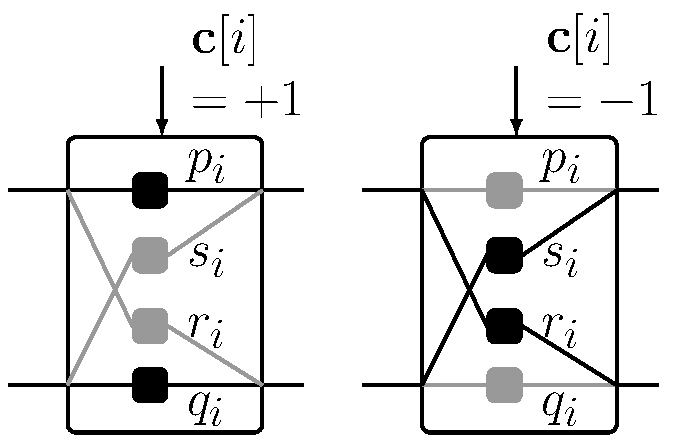
\includegraphics[width=.6\textwidth]{apuf_stage_delays_chal.pdf}

\caption{APUF's $i$-th stage}
\end{subfigure}%
\begin{subfigure}[b]{.4\textwidth}
\centering
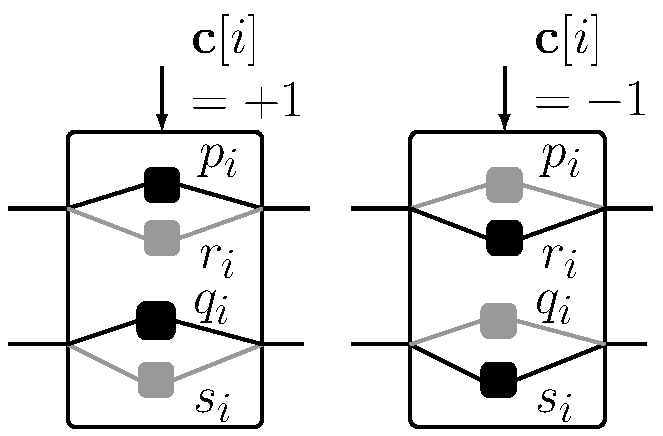
\includegraphics[width=.6\textwidth]{apuf_pdl_stage_delays_chal.pdf}
\caption{PAPUF's $i$-th stage}
\end{subfigure}

\caption{Switching stages of classic APUF and PAPUF. Depending on the challenge bit $\mathrm{\mathbf {c}}[i] \in \{+1,-1\}$, a pair of delay elements is selected.}

\end{figure}



\question Figure~\ref{fig:SMS4} shows the structure of a block cipher SMS4. Figure~\ref{fig:SMS4}(a) shows one round of the cipher, while 
Figure~\ref{fig:SMS4}(b) shows 4 rounds of the cipher. 
The inputs to round $i$ $(0 \le i \le 31)$ are four $32$ bit words $X_i,X_{i+1},X_{i+2},X_{i+3}$, 
and a round key $RK_i$, which also of size $32$ bits. 
In each round, the 32-bit inputs ($X_i$) and round key $RK_i$ are divided into
4 parts, each of 8 bits. These are respectively denoted $X_{i,0}$, $X_{i,1}$, $X_{i,2}$, 
$X_{i,3}$ and
$RK_{i,0}, RK_{i,1}, RK_{i,2}, RK_{i,3}$.

\begin{figure}[h]
	\centering
	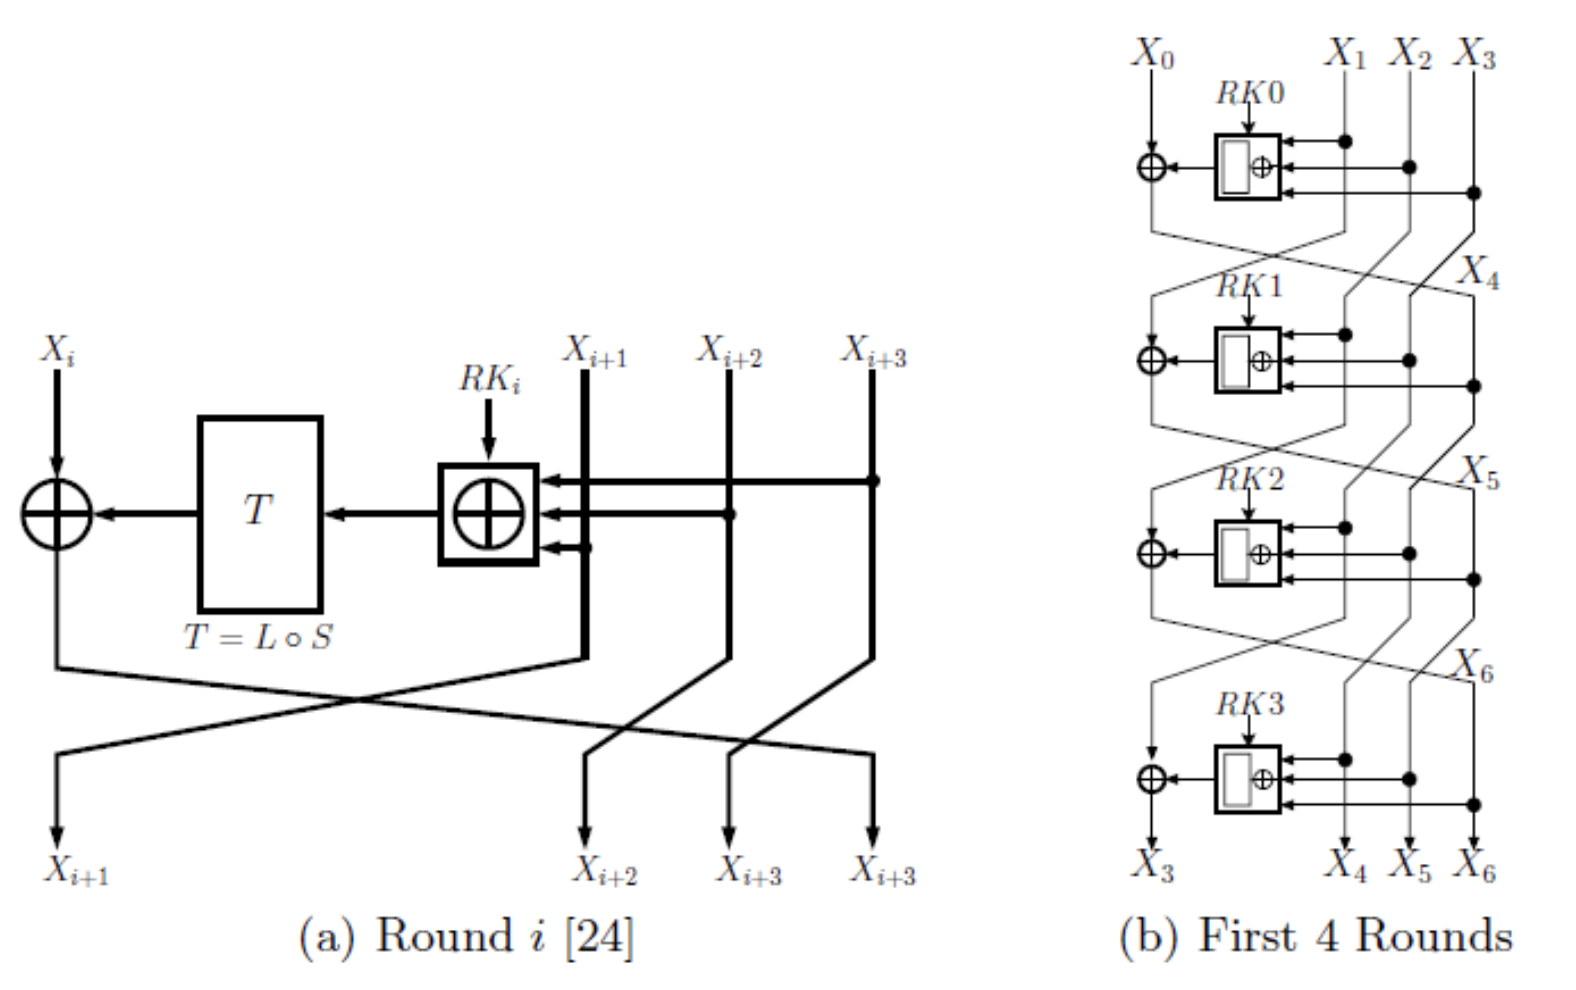
\includegraphics[scale=0.4]{SMS4.png}
    \caption{Round Structure of SMS4}
    \label{fig:SMS4}
\end{figure}

Each round of SMS4 generates the word $X_{i+4}$ as:\\
$X_{i+4} = F(X_i,X_{i+1},X_{i+2},X_{i+3})
= X_i \oplus T(X_{i+1} \oplus X_{i+2} \oplus X_{i+3} \oplus {RK_i})$\\. 
The transformation $T$ is a composition of S-Boxes ($S$) and diffusion layer ($L$). 
You do not need the details of the layer $L$. The layer $S$ is made of 
$4$ smaller and same s-boxes of dimension $8 \times 8$ each. 
The s-box is implemented as 
a table in the software implementation of the cipher, 
and thus leads to cache hit-misses. 

The round function has thus 4 cache accesses from each of the four words of $X_{i+1},X_{i+2}, X_{i+3}$. 
For example, the first access to the 
s-box is $X_{1,0} \oplus X_{2,0} \oplus X_{3,0} \oplus RK_{0,0}$.

\begin{enumerate}
\item Let a plaintext $(X_0 , X_1 , X_2 , X_3)$ be chosen such that there are 7 cache hits out of the 8 table accesses in the first 2 rounds (Note that the first memory access can never be a cache hit by the assumption of a flushed cache at the start of encryption). Derive the cache collision equations for Round-0 and Round-1. 

\marks{6}

\item Let P = $(X_0 , X_1 , X_2 , X_3)$ and $\hat{P} = (\hat{X_0}, \hat{X_1},\hat{X_2},\hat{X_3})$ be two such plaintexts which satisfy your derived equations and $P \neq \hat{P}$. This set of equations help in removing wrong candidates of RK0. 
Derive the equations in such scenario.

\marks{6}

\item Provide an estimate to the number of plaintext pairs $(P,\hat{P})$ required to uniquely retrieve RK0. Assume that the cache line is of size $m$ bytes, and the table used to implement the s-box is of $2^l$ bytes. The number of most significant bits revealed from each cache access is therefore $n = l - log_2m$.

\marks{3}
\end{enumerate}






\end{questions}






\end{document}


